\chapter{Method of work}
\label{chap:method}
\drop{I}{n} this chapter, the development software methodology during the
development of Geo-Cloud is described. Also, the tools such hardware and software used for is depicted.
 
\section{Development Methodology}
The selected methodology has been the \emph{iterative and incremental}
model. This model provides numerous advantages as early adaptability, testing
continuously and to have a implementation quite close to the final product. A
scheme of the model is shown in figure~\ref{fig:IncrementalModel}.


\begin{figure}[!h]
\begin{center}
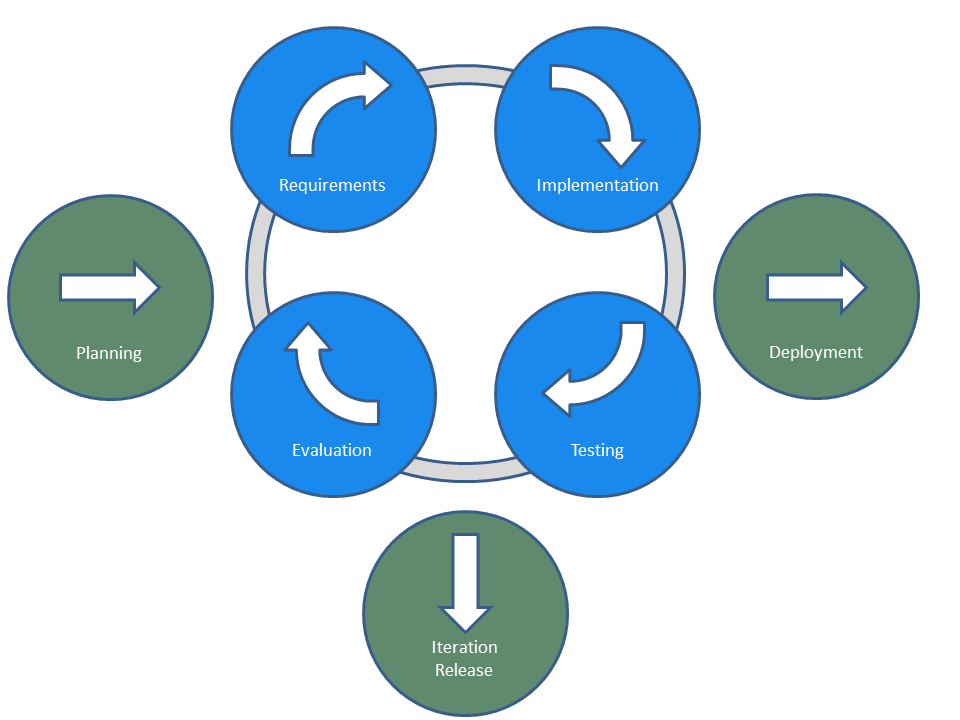
\includegraphics[width=0.7\textwidth]{statement/IterativeIncrementalDevelopment.png}
%http://www.meranetworks.com/services/processes/iterative
\caption{Iterative-incremental model}
\label{fig:IncrementalModel}
\end{center}
\end{figure}

This methodology enforces a strategy based in small iterations in which ones
there are short changes applies to each module. This permits to generate a prototype
growing and closing to the final version validating the initial requirements. In
this way if any changes are required by the advisor, is easily to carry out
them.
 
As the project has several parts, it is divided in modules and simultaneously,
each module is divided in iterations. These iterations are depicted in Section~\ref{section:evolution}.

\section{Tools}

In this section the resources such as software and hardware used during the
development are enumerated and described.  



\subsection{Programming Languages}

Several programming languages have been used for the Geo-Cloud
implementation. These languages are described in Section~\ref{sec:high-level-languages} and they can be
summarized as follows:

\begin{itemize}
\item \textbf{Python:}  Main language used in the project. It is a
  multiplatform, multipurpose object oriented language, although permits imperative and functional
programming. It does not need to compile the source because it is
interpreted (the operative systems in the cloud maybe not the same).
 \item \textbf{\ac{XML}:} is a mark-up language that defines a set of rules for encoding
documents in a format. It is used in some configuration files used by the
   Orchestrator module or the User Interface tool.

\item \textbf{\ac{JSON}:} is a lightweight language for data interchange between
  applications. The \bonfire experiment descriptor must be written in this
  language indicating the virtual machines instances, physical machines and the
  network resources instantiated.

\item \textbf{Bash:}  consists of several sentences that the operative system is
able to read and translate in order to play a specific action. All the currents
\emph{Linux} distributions contains a Bash interpret. 

\end{itemize}


\subsection{Hardware}

The development of GEO-Cloud project has been carried out in a PC owned by
Deimos with the following features:
\begin{itemize}
\item \emph{Intel Core i5 3450 3.1 GHz}
\item \emph{8 GB RAM}
\end{itemize}

For the Version Control, the chosen server is
Bitbucket~\footnote{http:www.bitbucket.org}.

The used resources provided  by the \emph{Fed4FIRE} testbeds are the following:

\begin{itemize}
\item \textbf{PlanetLab}: It currently provides 1204 nodes at 593 sites around
  the world. The selected nodes for carrying out this project are shown in
  Table~\ref{tab:ple-tablelayer1-nodes} and Table~\ref{tab:ple-tablelayer2-nodes}.

\item \textbf{Virtual Wall}: It consists of 100 nodes (dual processor o dual
  core servers) interconnected via a non-blocking 1.5 Tb/s Ethernet switch. 29
  nodes have been used to simulate the satellite constellation and ground
  stations. 

\item \textbf{BonFIRE}: Nodes from diferent testbeds have been selected. The
  features of each node are depicted in Table~\ref{table:intro-instance-types} 
  \begin{itemize}
    \item From INRIA: 2 nodes Medium.
    \item From EPCC: 1 node Xlarge for Orchestrator and a \ac{EaaS} for
      Processing Chain with at least 1  and maximum 60 active Xlarge resources. <<MODIFICABLE>>
    \item From IBBT: 1 Shared Storage.

    \end{itemize}
\end{itemize}


\subsection{Software}

Then, the tools and libraries used for the project are depicted:

\begin{itemize}
\item \textbf{Operative Systems}
\begin{itemize}
\item{\emph{Ubuntu}}: UNIX based operative system in which the development has done. It
  is based in Debian and distributed under \ac{GPL} v3.
\item{\emph{Debian}}: UNIX based operative system distributed under \ac{GPL}
  v3. It provides more than 37500 precompiled software packets which can be
  installed easily. The \bonfire, \vw and \pl machines run this operative system.
\end{itemize}
\item \textbf{Software Development Tools}

\begin{itemize}
\item{\emph{Emacs}}: versatile and powerful text editor developed by Richard
  Stallman. This tool is used with \emph{Pymacs} together. Version used 23.2.
\item{\emph{JFed}}: tool developed by \emph{IMinds} (University of
  Gent)\footnote{http:www.jfed.iminds.be} for deploying nodes from
  \emph{Fed4FIRE} testbeds. 
\item{\emph{BonFIRE Web Interface}}: \bonfire tool that provides the experiment
  deployment manually or to upload an experiment descriptor for automatic
  deployment.
\item \emph{Ipython:}  command shell for interactive computing in Python. It
  allows to check some clauses before adding it into a software. For agile
  development, it is a useful tool. 
\end{itemize}


\item \textbf{Graphics and documentation}

\begin{itemize}
%http://www.latex-project.org/
\item{\emph{\LaTeX}}:is a document mark-up language widely used for the
  communication and publication of scientific documents. It is multiplatform and is distributed under \ac{GPL} v3.
%http://www.gimp.org/
\item{\emph{GIMP}}: is the \emph{GNU Image Manipulation Program}. It allows some
  achievements as photo retouching, image composition and image authoring among
  others. It is multiplatform and is distributed under \ac{GPL} v3.
%http://dia-installer.de/index.html.es
\item{\emph{Dia}}: multiplatform software for drawing many types of
  schemes. Some design schemes of this document were performed on it.
% https://en.libreoffice.org/
\item \emph{Libre Office:} free open source office suite, developed by \emph{The
      Document Foundation}. This suite provides such software as \emph{Draw} and
    \emph{Writer} among other programs. 
\end{itemize}

\item \textbf{Software Libraries}

\begin{itemize}
\item{\emph{Python-mysql}}: \emph{Python} library that provides a high-level interface
  \emph{MySQL} programming. 
\item{\emph{Python-mathplotlib}}: \emph{Python} library that provides some tools and
  functions for plotting and representing data. 
\item{\emph{Python-xml}}:\emph{Python} library used to manage \ac{XML} files.
\item{\emph{Paramiko}}: \emph{Python} library that provides high-level interfaces for
  connecting through \ac{SSH} to other network host. 
\item \emph{PyQt:} Python binding for the \emph{Qt} cross-platform framework. \emph{PyQt} is
  available in two versions, \emph{PyQt4} and \emph{PyQt5}. \emph{PyQt5} was used for developing the
  project. 
\item \emph{Phonon:} multimedia \ac{API} provided by Qt for handling multimedia
  streams. For developing the \ac{GUI} of this project, this library was used.
\end{itemize}
\end{itemize}
